\documentclass[12pt,twoside]{report}
\usepackage[utf8]{inputenc}
\usepackage{setspace}
\usepackage{graphicx}
\usepackage[a4paper, width=150mm,top=25mm,bottom=25mm,bindingoffset=6mm]{geometry}
\usepackage{fancyhdr}
\usepackage[page]{totalcount}
\usepackage{caption}
\usepackage{subcaption}
\usepackage[nottoc]{tocbibind}
% \usepackage[fit]{truncate}



\newcommand{\changefont}{
    \fontsize{9}{11}\selectfont
}
\pagestyle{fancy}
\fancyhead{}

\fancyhead[RE]{\changefont \leftmark}
\fancyhead[LO]{\changefont \rightmark}

\fancyfoot{}
\fancyfoot[LO, RE]{\thepage}

\renewcommand{\headrulewidth}{0.7pt}
% \fancyhead[LO, RE]{Page \textbf{\thepage} ~of \totalpages}

\graphicspath{ {images/} }

\title{
    {A Las vegas algorithm to solve Elliptic Curve Discrete Logarithm Problem in public key cryptography}\\
    {\large Interdisciplinary School of Scientific Computing - SPPU}\\
    
\includegraphics[width=0.2\textwidth]{issc.jpg}
}
\author{Author Name}
\date{Day Month Year}

% \doublespacing
\onehalfspacing
\begin{document}

\maketitle

\pagenumbering{roman}                             % small roman letters as page numbers
\chapter*{Dedication}
To Mum and Dad...family and friends and unknow people on the internet...


\chapter*{Certificate of the GUIDE}
This is to certify, that the work done in this thesis "A las vegas algorithm to solve elliptic curve discrete logarithm problem in public key cryptography" submitted by Abdullah Zubair Ansari, was carried out by the candidate under out guidance. The work incorporated in this thesis has not been submitted to any other University or Institute for the degree of Ph.D. or any other degree or academic award. Such materialsm as had been obtained from other sources, have be dualy acknowledged in the thesis


\chapter*{Declaration}
I declare that the thesis titled \textbf{"A Las Vegas algorithm to solve Elliptic Curve Discrete Logarithm problem in public key cryptography"} submitted by me for the degree of Doctor of Philosophy is the record of word carried out by me during the period from January 2016 to JUNE 2021 under the guidance of Dr. Smita Bedekar (ISSC-SPPU) and Dr. Ayan Mahanalobis (IISER-PUNE) and had not formed the basis for the award of any degree, diploma, associateship, fellowship, titles in this or any other University or the other institution of Higher learning. I further declare that the material obtained from other sources had been duly acknowledged in the thesis.


\chapter*{Acknowledgement}
Lorem Ipsum is simply dummy text of the printing and typesetting industry. Lorem Ipsum has been the industry's standard dummy text ever since the 1500s, when an unknown printer took a galley of type and scrambled it to make a type specimen book. It has survived not only five centuries, but also the leap into electronic typesetting, remaining essentially unchanged. It was popularised in the 1960s with the release of Letraset sheets containing Lorem Ipsum passages, and more recently with desktop publishing software like Aldus PageMaker including versions of Lorem Ipsum.



% TODO : Format TOC i.e. decorate it a bit, line-spacing etc.
\tableofcontents

\listoffigures
\pagenumbering{arabic}

\listoftables

% TODO : Add list of Abbreviations to TOC
\chapter*{List of Abbreviations}

\chapter{An Introduction }

\section{Introduction}

An ability to have a secure communication medium has been of human interest since time immemorial.
A medium is secure for communication if it allows information flow between two entities such that, even if any third person 
gains access to this channel the information flowing is of no use to that person.
For the information to be useless for any third person it has to be converted to a form that makes no sense for any third person.
This conversion process is known as encryption and the converted message as ciphertext. 
The process of getting back the original message from ciphertext is decryption.
Thus,

\begin{center}
$\displaystyle
        Cryptography  = Encryption + Decryption. 
$
\end{center}

The idea of Public Key Cryptosystem was proposed by Diffie and Hellman in 1976. Since then a number of cryptosystems have been proposed.
Public key cryptographic protocols used in practical applications are based on some known mathematical hard problems.
RSA is based on the \textbf{I}nteger \textbf{F}actorization \textbf{P}roblem (IFP), ElGamal is based on the \textbf{D}iscrete \textbf{L}og 
\textbf{P}roblem (DLP) and the \cite{einstein}
\textbf{E}lliptic \textbf{C}urve \textbf{C}ryptosystem (ECC) are based over the Discrete Log Problem in a group of points over an elliptic curve.

\begin{figure}[h]
\centering
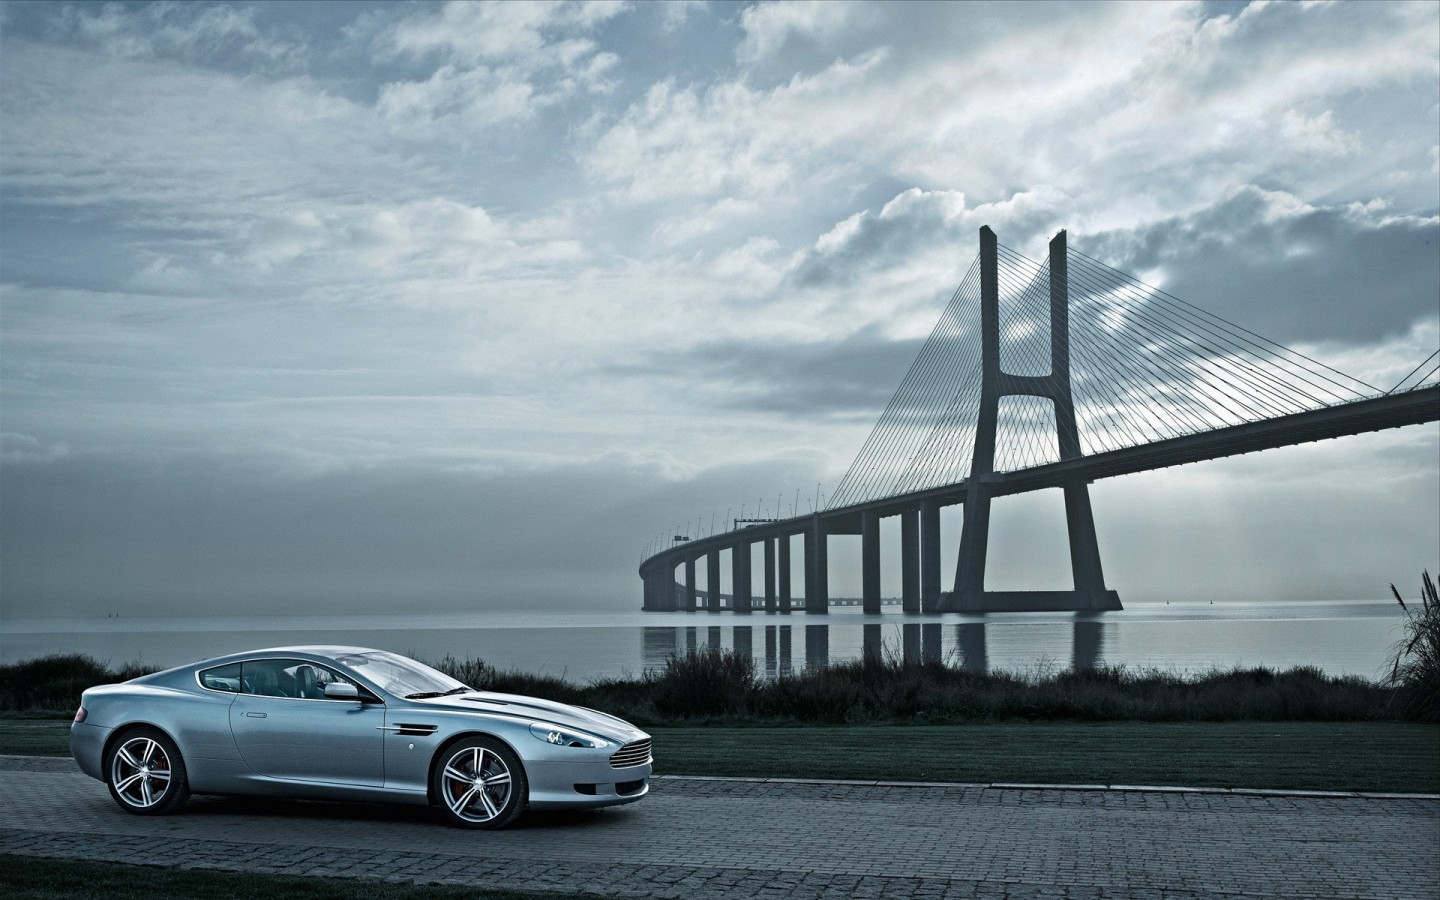
\includegraphics[scale=0.3]{DB9}
\caption{ASTON MARTIN DB9}
\label{DB9}
\end{figure}

Recent see \ref{DB9} advances in the index calculus attack for DLP by Joux have shown that the cryptosystems over a finite field of small characteristics are no longer
secure.
A Quasi-polynomial time algorithm to solve the DLP in a multiplicative group of finite extension field was proposed by Joux in. Since then the DLP
is not as hard to solve as it used to be in some setting.

Index calculus algorithms are not suitable for for solving DLP efficiently in an elliptic curve group.
Thus only attacks available for the DLP over elliptic curve are the generic algorithms like the Pollard rho or the r-adding walk.
The time complexity for these algorithms is about the square root of the size of the group.

As a result of the advancement in the index calculus attack for fields with small characteristics, the set of cryptographic algorithms
proposed in ``Suite B Cryptography''  by the National Security Agency (USA) recommends ECC.
Thus currently, there is no other highly recommended public key cryptosystem other than the ECC in use for practical applications.
Public key Cryptosystems based on finite fields are over small characteristics, mostly binary field, i.e characteristic 2.
As binary fields are similar to the binary nature of a digital computer there are extremely efficient algorithms for 
performing operations over the field elements. 
Hence, cryptosystems over fields of characteristic greater than 2 were never needed in practice.\newline
Thus to summarize the present situation in public key cryptography :-

\begin{itemize}
  \item No recommended Public key cryptosystem other than ECC
  \item Non-ECC over small characteristics are not secure for practical applications
\end{itemize}

As no cryptosystem other than Elliptic curve cryptosystem is available for higher characteristic we aim to develop a new public-key
cryptosystem based on the Discrete Log Problem for higher characteristics.
This system would be based on the DLP over circulant matrices which are defined over a finite field of large characteristic.
A cryptosystem based on characteristic 2 fields was proposed in.
Cryptographic protocols based over any general or a special type of matrices are not used in everyday cryptography.
Generally, it is believed that matrices offer no major security or efficiency advantage.
Here we would be working with matrices of a special type.
These matrices have a certain structure in them, using this structure matrix operations can be performed in an efficient manner.
These matrices can provide security and computational efficiency as compared to systems over finite fields used today in public key cryptography.


\section{Cryptosystem to be implemented}

\subsection{Circulant matrices}
An $n \times n$ matrix C is a circulant matrix if all its rows (or columns) other than the first are a circular shift of the previous
row (or column).

\[ C =\left( \begin{array}{ccccc}
c_{0} & c_{1}   &  \cdots  &c_{n-2} & c_{n-1} \\
c_{n-1} & c_{0}  &  \cdots  &c_{n-3}    &c_{n-2} \\
c_{n-2} & c_{n-1}     &  \cdots  &c_{n-4}  &c_{n-3} \\
\vdots   &\vdots  & \ddots& \vdots   & \vdots \\
c_{1} & c_{2}   &  \cdots  &c_{n-1}   &c_{0}
\end{array} \right)\]

An $n \times n$ circulant matrix has atmost $n$ different entries and can be determined completly by the first row, i.e.
% $\text{C} = \text{circ}(c_{0}, c_{1},c_{2},c_{3},... c_{n-1}).$
A circulant matrix is a special case of the Toeplitz matrix which is a square matrix with constant diagonals.
Even though a matrix is a 2-dimensional entity, due to the structure of a circulant matrix it behaves like a one-dimensional array. Thus
allowing operations on the matrix to be performed in an efficient manner.
Circulant matrices form a commutative ring under matrix multiplication and addition.

\subsection{ElGamal cryptosystem}
The ElGamal Cryptosystem is a public key cryptosystem based on the discrete logarithm in a group $ G $.
Given a primitive element a $ \in $ G and another element b, DLP is the computational problem of finding 
$x = log_{a} (b) $ such that $b = a^{x}$.

\subsection{Discrete Logarithm problem in matrices}
The DLP in matrices is to find $m$, from $A$ and $A^m$ where $A$ $\in$ $GL(d,q)$.
Here $GL(d,q)$ is a group of nonsingular matrices of size d over the finite field F

\subsection{Aim}

We will work with circulant matrices and ElGamal cryptosystem, to determine how fast one can do computations with circulant matrices
when implemented in a \textbf{C}omputer \textbf{A}lgebra \textbf{S}ystem (CAS) like Victor Shoup's 
\textbf{N}umber \textbf{T}heory \textbf{L}ibrary (NTL). 
How this cryptosystem will behave with finite fields of higher characteristics will be interesting as public key cryptosystems have never been 
implemented over finite fields of large characteristics.

How much secure this cryptosystem is? Is the cryptosystem secure for large characteristic?
Is it efficient than the cryptosystem implemented over a finite field for large characteristic?
These will be some of the questions to be answered during the course of the work.

Exponentiation is the fundamental operation required for the ElGamal cryptosystem.
Developing a cryptosystem over ElGamal with circulant matrices will require implementing exponentiation in circulant matrices.
Exponentiation over matrices is available in NTL.
However this implementation is for generic matrices, i.e structure of the matrix is not used for exponentiation computation.
One of the better-known algorithm for exponentiation computation is the square and multiply algorithm.
The two fundamental operations here are squaring and multiplication.
It is known that squaring is computationally free for finite fields of characteristic 2 using normal basis.
How fast can matrix multiplication be done in this case is a question that we will try to answer.
For a finite field of higher characteristic ($>$2), squaring is not computationally free.
How fast one can perform squaring and multiplication of circulant matrices in these fields will be another question to be answered.

Generating secure instances of circulant matrices to support the validity of the cryptosystem will be needed.
This is a computationally demanding task.
Computational complexity increases exponentially as size of the field increases.

The ElGamal cryptosystem works with any type of matrices. 
Circulant matrices were chosen because they have a structure which makes them interesting from the cryptographic perspective.
Similar generalization of circulant matrices are the Block circulant matrices, which too have some structure.
The structure here applies to the blocks rather than the elements of the matrix.

\section{Study the generalization of circulant matrices}

As there is a structure in Block circulant matrices it would be interesting to study them with the objective of using them to 
develop a public key cryptosystem.
Parallel matrix multiplication algorithms operate on matrices by dividing the input matrix into blocks and distributing these blocks onto 
different processors to get the multiplication done.
As block circulant matrices have an internal structure implementing them in a parallel environment can improve the efficiency of multiplication.
Thus, block circulant matrices can extract advantage from a parallel implementation, whereas for finite field implementation parallelization
is not straightforward.
The three generalization of the circulant matrix are:
\begin{itemize}
  \item Block Circulant matrices with circular blocks
  \item Block Circulant matrices with non-circular block
  \item Non-Circulant matrices with circular block
\end{itemize}

\subsection{Block Circulant matrices with Circular Blocks (BCCB)}

\[ C_{1} =\left( \begin{array}{ccccccc}
c_{0} & c_{1} &c_{2} & \vline & c_{3} & c_{4} &c_{5}    \\
c_{2} & c_{0} &c_{1} & \vline & c_{5} & c_{3} &c_{4}    \\
c_{1} & c_{2} &c_{0} & \vline & c_{4} & c_{5} &c_{3}    \\
\hline
c_{3} & c_{4} &c_{5} & \vline & c_{0} & c_{1} &c_{2}    \\
c_{5} & c_{3} &c_{4} & \vline & c_{2} & c_{0} &c_{1}    \\
c_{4} & c_{5} &c_{3} & \vline & c_{1} & c_{2} &c_{0}    \\
\end{array} \right)\]

A BCCB is not a circular matrix, the blocks are circular and each block row is a circular shift of the previous block row. 
In the example above $C_{1}$ is a BCCB with two $3 \times 3$ circular blocks, each block is a circular matrix in itself. 

\subsection{Block Circulant matrices with non-circular block}

\[ C_{2} =\left( \begin{array}{ccccccc}
c_{0} & c_{1} &c_{2} & \vline & c_{3} & c_{4} &c_{5} \\
c_{2} & c_{0} &c_{1} & \vline & c_{5} & c_{3} &c_{4} \\
c_{1} & c_{2} &c_{0} & \vline & c_{4} & c_{5} &c_{3} \\
\hline
c_{6} & c_{7} &c_{8} & \vline & c_{9} & c_{10} &c_{11} \\
c_{8} & c_{6} &c_{7} & \vline & c_{11} & c_{9} &c_{10} \\
c_{7} & c_{8} &c_{6} & \vline & c_{10} & c_{11} &c_{9} \\
\end{array} \right)\]

In block circulant matrix with non-circular block the blocks  themselves are circular. The matrix is not circular. Thus  a row from
each block is required to represent the entire matrix.

\subsection{Non-Circulant matrices with circular block}
\[ C_{3} =\left( \begin{array}{ccccccc}
c_{0} & c_{1} &c_{2} & \vline & c_{9} & c_{10} &c_{11}   \\
c_{3} & c_{4} &c_{5} & \vline & c_{12} & c_{13} &c_{14}   \\
c_{6} & c_{7} &c_{8} & \vline & c_{15} & c_{16} &c_{17}   \\
\hline
c_{9} & c_{10} &c_{11} & \vline & c_{0} & c_{1} &c_{2}   \\
c_{12} & c_{13} &c_{14} & \vline & c_{3} & c_{4} &c_{5}  \\
c_{15} & c_{16} &c_{17} & \vline & c_{6} & c_{7} &c_{8}   \\
\end{array} \right)\]

In non-circulant matrix with circular block the blocks themselves are not circular nor is the matrix a circulant matrix. 
Each block row is a circular shift of the previous block row.


\chapter[ECDLP]{Algorithms to solve ECDLP }

\section[SEC-1]{Introduction Chapter 2}

An ability to have a secure communication medium has been of human interest since time immemorial.
A medium is secure for communication if it allows information flow between two entities such that, even if any third person 
gains access to this channel the information flowing is of no use to that person.
For the information to be useless for any third person it has to be converted to a form that makes no sense for any third person.
This conversion process is known as encryption and the converted message as ciphertext. 
The process of getting back the original message from ciphertext is decryption.
Thus,

\begin{center}
$\displaystyle
        Cryptography  = Encryption + Decryption. 
$
\end{center}

The idea of Public Key Cryptosystem was proposed by Diffie and Hellman in 1976. Since then a number of cryptosystems have been proposed.
Public key cryptographic protocols used in practical applications are based on some known mathematical hard problems.
RSA is based on the \textbf{I}nteger \textbf{F}actorization \textbf{P}roblem (IFP), ElGamal is based on the \textbf{D}iscrete \textbf{L}og 
\textbf{P}roblem (DLP) and the 
\textbf{E}lliptic \textbf{C}urve \textbf{C}ryptosystem (ECC) are based over the Discrete Log Problem in a group of points over an elliptic curve.

Recent advances in the index calculus attack for DLP by Joux have shown that the cryptosystems over a finite field of small characteristics are no longer
secure.
A Quasi-polynomial time algorithm to solve the DLP in a multiplicative group of finite extension field was proposed by Joux in. Since then the DLP
is not as hard to solve as it used to be in some setting.

Index calculus algorithms are not suitable for for solving DLP efficiently in an elliptic curve group.
Thus only attacks available for the DLP over elliptic curve are the generic algorithms like the Pollard rho or the r-adding walk.
The time complexity for these algorithms is about the square root of the size of the group.

As a result of the advancement in the index calculus attack for fields with small characteristics, the set of cryptographic algorithms
proposed in ``Suite B Cryptography''  by the National Security Agency (USA) recommends ECC.
Thus currently, there is no other highly recommended public key cryptosystem other than the ECC in use for practical applications.
Public key Cryptosystems based on finite fields are over small characteristics, mostly binary field, i.e characteristic 2.
As binary fields are similar to the binary nature of a digital computer there are extremely efficient algorithms for 
performing operations over the field elements. 
Hence, cryptosystems over fields of characteristic greater than 2 were never needed in practice.\newline
Thus to summarize the present situation in public key cryptography :-

\begin{itemize}
  \item No recommended Public key cryptosystem other than ECC
  \item Non-ECC over small characteristics are not secure for practical applications
\end{itemize}

As no cryptosystem other than Elliptic curve cryptosystem is available for higher characteristic we aim to develop a new public-key
cryptosystem based on the Discrete Log Problem for higher characteristics.
This system would be based on the DLP over circulant matrices which are defined over a finite field of large characteristic.
A cryptosystem based on characteristic 2 fields was proposed in.
Cryptographic protocols based over any general or a special type of matrices are not used in everyday cryptography.
Generally, it is believed that matrices offer no major security or efficiency advantage.
Here we would be working with matrices of a special type.
These matrices have a certain structure in them, using this structure matrix operations can be performed in an efficient manner.
These matrices can provide security and computational efficiency as compared to systems over finite fields used today in public key cryptography.

\section[ic]{Implementation of the Cryptosystem}

\subsection{Circulant matrices}
An $n \times n$ matrix C is a circulant matrix if all its rows (or columns) other than the first are a circular shift of the previous
row (or column).

\[ C =\left( \begin{array}{ccccc}
c_{0} & c_{1}   &  \cdots  &c_{n-2} & c_{n-1} \\
c_{n-1} & c_{0}  &  \cdots  &c_{n-3}    &c_{n-2} \\
c_{n-2} & c_{n-1}     &  \cdots  &c_{n-4}  &c_{n-3} \\
\vdots   &\vdots  & \ddots& \vdots   & \vdots \\
c_{1} & c_{2}   &  \cdots  &c_{n-1}   &c_{0}
\end{array} \right)\]

An $n \times n$ circulant matrix has atmost $n$ different entries and can be determined completly by the first row, i.e.
% $\text{C} = \text{circ}(c_{0}, c_{1},c_{2},c_{3},... c_{n-1}).$
A circulant matrix is a special case of the Toeplitz matrix which is a square matrix with constant diagonals.
Even though a matrix is a 2-dimensional entity, due to the structure of a circulant matrix it behaves like a one-dimensional array. Thus
allowing operations on the matrix to be performed in an efficient manner.
Circulant matrices form a commutative ring under matrix multiplication and addition.

\subsection{ElGamal cryptosystem}
The ElGamal Cryptosystem is a public key cryptosystem based on the discrete logarithm in a group $ G $.
Given a primitive element a $ \in $ G and another element b, DLP is the computational problem of finding 
$x = log_{a} (b) $ such that $b = a^{x}$.

\subsection{Discrete Logarithm problem in matrices}
The DLP in matrices is to find $m$, from $A$ and $A^m$ where $A$ $\in$ $GL(d,q)$.
Here $GL(d,q)$ is a group of nonsingular matrices of size d over the finite field F

\subsection{Aim}

We will work with circulant matrices and ElGamal cryptosystem, to determine how fast one can do computations with circulant matrices
when implemented in a \textbf{C}omputer \textbf{A}lgebra \textbf{S}ystem (CAS) like Victor Shoup's 
\textbf{N}umber \textbf{T}heory \textbf{L}ibrary (NTL). 
How this cryptosystem will behave with finite fields of higher characteristics will be interesting as public key cryptosystems have never been 
implemented over finite fields of large characteristics.

How much secure this cryptosystem is? Is the cryptosystem secure for large characteristic?
Is it efficient than the cryptosystem implemented over a finite field for large characteristic?
These will be some of the questions to be answered during the course of the work.

Exponentiation is the fundamental operation required for the ElGamal cryptosystem.
Developing a cryptosystem over ElGamal with circulant matrices will require implementing exponentiation in circulant matrices.
Exponentiation over matrices is available in NTL.
However this implementation is for generic matrices, i.e structure of the matrix is not used for exponentiation computation.
One of the better-known algorithm for exponentiation computation is the square and multiply algorithm.
The two fundamental operations here are squaring and multiplication.
It is known that squaring is computationally free for finite fields of characteristic 2 using normal basis.
How fast can matrix multiplication be done in this case is a question that we will try to answer.
For a finite field of higher characteristic ($>$2), squaring is not computationally free.
How fast one can perform squaring and multiplication of circulant matrices in these fields will be another question to be answered.

Generating secure instances of circulant matrices to support the validity of the cryptosystem will be needed.
This is a computationally demanding task.
Computational complexity increases exponentially as size of the field increases.

The ElGamal cryptosystem works with any type of matrices. 
Circulant matrices were chosen because they have a structure which makes them interesting from the cryptographic perspective.
Similar generalization of circulant matrices are the Block circulant matrices, which too have some structure.
The structure here applies to the blocks rather than the elements of the matrix.

\section{circulant matrices}

As there is a structure in Block circulant matrices it would be interesting to study them with the objective of using them to 
develop a public key cryptosystem.
Parallel matrix multiplication algorithms operate on matrices by dividing the input matrix into blocks and distributing these blocks onto 
different processors to get the multiplication done.
As block circulant matrices have an internal structure implementing them in a parallel environment can improve the efficiency of multiplication.
Thus, block circulant matrices can extract advantage from a parallel implementation, whereas for finite field implementation parallelization
is not straightforward.
The three generalization of the circulant matrix are:
\begin{itemize}
  \item Block Circulant matrices with circular blocks
  \item Block Circulant matrices with non-circular block
  \item Non-Circulant matrices with circular block
\end{itemize}

\subsection{Block Circulant matrices with Circular Blocks (BCCB)}

\[ C_{1} =\left( \begin{array}{ccccccc}
c_{0} & c_{1} &c_{2} & \vline & c_{3} & c_{4} &c_{5}    \\
c_{2} & c_{0} &c_{1} & \vline & c_{5} & c_{3} &c_{4}    \\
c_{1} & c_{2} &c_{0} & \vline & c_{4} & c_{5} &c_{3}    \\
\hline
c_{3} & c_{4} &c_{5} & \vline & c_{0} & c_{1} &c_{2}    \\
c_{5} & c_{3} &c_{4} & \vline & c_{2} & c_{0} &c_{1}    \\
c_{4} & c_{5} &c_{3} & \vline & c_{1} & c_{2} &c_{0}    \\
\end{array} \right)\]

A BCCB is not a circular matrix, the blocks are circular and each block row is a circular shift of the previous block row. 
In the example above $C_{1}$ is a BCCB with two $3 \times 3$ circular blocks, each block is a circular matrix in itself. 

\subsection{Block Circulant matrices with non-circular block}

\[ C_{2} =\left( \begin{array}{ccccccc}
c_{0} & c_{1} &c_{2} & \vline & c_{3} & c_{4} &c_{5} \\
c_{2} & c_{0} &c_{1} & \vline & c_{5} & c_{3} &c_{4} \\
c_{1} & c_{2} &c_{0} & \vline & c_{4} & c_{5} &c_{3} \\
\hline
c_{6} & c_{7} &c_{8} & \vline & c_{9} & c_{10} &c_{11} \\
c_{8} & c_{6} &c_{7} & \vline & c_{11} & c_{9} &c_{10} \\
c_{7} & c_{8} &c_{6} & \vline & c_{10} & c_{11} &c_{9} \\
\end{array} \right)\]

In block circulant matrix with non-circular block the blocks  themselves are circular. The matrix is not circular. Thus  a row from
each block is required to represent the entire matrix.

\subsection{Non-Circulant matrices with circular block}
\[ C_{3} =\left( \begin{array}{ccccccc}
c_{0} & c_{1} &c_{2} & \vline & c_{9} & c_{10} &c_{11}   \\
c_{3} & c_{4} &c_{5} & \vline & c_{12} & c_{13} &c_{14}   \\
c_{6} & c_{7} &c_{8} & \vline & c_{15} & c_{16} &c_{17}   \\
\hline
c_{9} & c_{10} &c_{11} & \vline & c_{0} & c_{1} &c_{2}   \\
c_{12} & c_{13} &c_{14} & \vline & c_{3} & c_{4} &c_{5}  \\
c_{15} & c_{16} &c_{17} & \vline & c_{6} & c_{7} &c_{8}   \\
\end{array} \right)\]

In non-circulant matrix with circular block the blocks themselves are not circular nor is the matrix a circulant matrix. 
Each block row is a circular shift of the previous block row.


\section{Introduction Study the generalization of }

An ability to have a secure communication medium has been of human interest since time immemorial.
A medium is secure for communication if it allows information flow between two entities such that, even if any third person 
gains access to this channel the information flowing is of no use to that person.
For the information to be useless for any third person it has to be converted to a form that makes no sense for any third person.
This conversion process is known as encryption and the converted message as ciphertext. 
The process of getting back the original message from ciphertext is decryption.
Thus,

\begin{center}
$\displaystyle
        Cryptography  = Encryption + Decryption. 
$
\end{center}

The idea of Public Key Cryptosystem was proposed by Diffie and Hellman in 1976. Since then a number of cryptosystems have been proposed.
Public key cryptographic protocols used in practical applications are based on some known mathematical hard problems.
RSA is based on the \textbf{I}nteger \textbf{F}actorization \textbf{P}roblem (IFP), ElGamal is based on the \textbf{D}iscrete \textbf{L}og 
\textbf{P}roblem (DLP) and the 
\textbf{E}lliptic \textbf{C}urve \textbf{C}ryptosystem (ECC) are based over the Discrete Log Problem in a group of points over an elliptic curve.

Recent advances in the index calculus attack for DLP by Joux have shown that the cryptosystems over a finite field of small characteristics are no longer
secure.
A Quasi-polynomial time algorithm to solve the DLP in a multiplicative group of finite extension field was proposed by Joux in. Since then the DLP
is not as hard to solve as it used to be in some setting.

Index calculus algorithms are not suitable for for solving DLP efficiently in an elliptic curve group.
Thus only attacks available for the DLP over elliptic curve are the generic algorithms like the Pollard rho or the r-adding walk.
The time complexity for these algorithms is about the square root of the size of the group.

As a result of the advancement in the index calculus attack for fields with small characteristics, the set of cryptographic algorithms
proposed in ``Suite B Cryptography''  by the National Security Agency (USA) recommends ECC.
Thus currently, there is no other highly recommended public key cryptosystem other than the ECC in use for practical applications.
Public key Cryptosystems based on finite fields are over small characteristics, mostly binary field, i.e characteristic 2.
As binary fields are similar to the binary nature of a digital computer there are extremely efficient algorithms for 
performing operations over the field elements. 
Hence, cryptosystems over fields of characteristic greater than 2 were never needed in practice.\newline
Thus to summarize the present situation in public key cryptography :-


\chapter{The LasVegas Algorithm }
\section{Introduction}
Lorem Ipsum is simply dummy text of the printing and typesetting industry. Lorem Ipsum has been the industry's standard dummy text ever since the 1500s, when an unknown printer took a galley of type and scrambled it to make a type specimen book. It has survived not only five centuries, but also the leap into electronic typesetting, remaining essentially unchanged. It was popularised in the 1960s with the release of Letraset sheets containing Lorem Ipsum passages, and more recently with desktop publishing software like Aldus PageMaker including versions of Lorem Ipsum.


\section{Introduction}
Lorem Ipsum is simply dummy text of the printing and typesetting industry. Lorem Ipsum has been the industry's standard dummy text ever since the 1500s, when an unknown printer took a galley of type and scrambled it to make a type specimen book. It has survived not only five centuries, but also the leap into electronic typesetting, remaining essentially unchanged. It was popularised in the 1960s with the release of Letraset sheets containing Lorem Ipsum passages, and more recently with desktop publishing software like Aldus PageMaker including versions of Lorem Ipsum.


\subsection{Introduction}
Lorem Ipsum is simply dummy text of the printing and typesetting industry. Lorem Ipsum has been the industry's standard dummy text ever since the 1500s, when an unknown printer took a galley of type and scrambled it to make a type specimen book. It has survived not only five centuries, but also the leap into electronic typesetting, remaining essentially unchanged. It was popularised in the 1960s with the release of Letraset sheets containing Lorem Ipsum passages, and more recently with desktop publishing software like Aldus PageMaker including versions of Lorem Ipsum.


\chapter{Schur Complement to solve ECDLP }
\section{Introduction}
Lorem Ipsum is simply dummy text of the printing and typesetting industry. Lorem Ipsum has been the industry's standard dummy text ever since the 1500s, when an unknown printer took a galley of type and scrambled it to make a type specimen book. It has survived not only five centuries, but also the leap into electronic typesetting, remaining essentially unchanged. It was popularised in the 1960s with the release of Letraset sheets containing Lorem Ipsum passages, and more recently with desktop publishing software like Aldus PageMaker including versions of Lorem Ipsum.


\section{Introduction}
Lorem Ipsum is simply dummy text of the printing and typesetting industry. Lorem Ipsum has been the industry's standard dummy text ever since the 1500s, when an unknown printer took a galley of type and scrambled it to make a type specimen book. It has survived not only five centuries, but also the leap into electronic typesetting, remaining essentially unchanged. It was popularised in the 1960s with the release of Letraset sheets containing Lorem Ipsum passages, and more recently with desktop publishing software like Aldus PageMaker including versions of Lorem Ipsum.


\subsection{Introduction}
Lorem Ipsum is simply dummy text of the printing and typesetting industry. Lorem Ipsum has been the industry's standard dummy text ever since the 1500s, when an unknown printer took a galley of type and scrambled it to make a type specimen book. It has survived not only five centuries, but also the leap into electronic typesetting, remaining essentially unchanged. It was popularised in the 1960s with the release of Letraset sheets containing Lorem Ipsum passages, and more recently with desktop publishing software like Aldus PageMaker including versions of Lorem Ipsum.


\chapter{Extension Minor, Maximal Minor, minus-3 hypothesis  }
\section{Introduction}
Lorem Ipsum is simply dummy text of the printing and typesetting industry. Lorem Ipsum has been the industry's standard dummy text ever since the 1500s, when an unknown printer took a galley of type and scrambled it to make a type specimen book. It has survived not only five centuries, but also the leap into electronic typesetting, remaining essentially unchanged. It was popularised in the 1960s with the release of Letraset sheets containing Lorem Ipsum passages, and more recently with desktop publishing software like Aldus PageMaker including versions of Lorem Ipsum.


\section{Introduction}
Lorem Ipsum is simply dummy text of the printing and typesetting industry. Lorem Ipsum has been the industry's standard dummy text ever since the 1500s, when an unknown printer took a galley of type and scrambled it to make a type specimen book. It has survived not only five centuries, but also the leap into electronic typesetting, remaining essentially unchanged. It was popularised in the 1960s with the release of Letraset sheets containing Lorem Ipsum passages, and more recently with desktop publishing software like Aldus PageMaker including versions of Lorem Ipsum.


\subsection{Introduction}
Lorem Ipsum is simply dummy text of the printing and typesetting industry. Lorem Ipsum has been the industry's standard dummy text ever since the 1500s, when an unknown printer took a galley of type and scrambled it to make a type specimen book. It has survived not only five centuries, but also the leap into electronic typesetting, remaining essentially unchanged. It was popularised in the 1960s with the release of Letraset sheets containing Lorem Ipsum passages, and more recently with desktop publishing software like Aldus PageMaker including versions of Lorem Ipsum.


\chapter{Conclusion }
\section{Introduction}
Lorem Ipsum is simply dummy text of the printing and typesetting industry. Lorem Ipsum has been the industry's standard dummy text ever since the 1500s, when an unknown printer took a galley of type and scrambled it to make a type specimen book. It has survived not only five centuries, but also the leap into electronic typesetting, remaining essentially unchanged. It was popularised in the 1960s with the release of Letraset sheets containing Lorem Ipsum passages, and more recently with desktop publishing software like Aldus PageMaker including versions of Lorem Ipsum.


\section{Introduction}
Lorem Ipsum is simply dummy text of the printing and typesetting industry. Lorem Ipsum has been the industry's standard dummy text ever since the 1500s, when an unknown printer took a galley of type and scrambled it to make a type specimen book. It has survived not only five centuries, but also the leap into electronic typesetting, remaining essentially unchanged. It was popularised in the 1960s with the release of Letraset sheets containing Lorem Ipsum passages, and more recently with desktop publishing software like Aldus PageMaker including versions of Lorem Ipsum.


\subsection{Introduction}
Lorem Ipsum is simply dummy text of the printing and typesetting industry. Lorem Ipsum has been the industry's standard dummy text ever since the 1500s, when an unknown printer took a galley of type and scrambled it to make a type specimen book. It has survived not only five centuries, but also the leap into electronic typesetting, remaining essentially unchanged. It was popularised in the 1960s with the release of Letraset sheets containing Lorem Ipsum passages, and more recently with desktop publishing software like Aldus PageMaker including versions of Lorem Ipsum.


\chapter*{List of publications}

\appendix
\chapter{How to use the code}
\section{Introduction}
Lorem Ipsum is simply dummy text of the printing and typesetting industry. Lorem Ipsum has been the industry's standard dummy text ever since the 1500s, when an unknown printer took a galley of type and scrambled it to make a type specimen book. It has survived not only five centuries, but also the leap into electronic typesetting, remaining essentially unchanged. It was popularised in the 1960s with the release of Letraset sheets containing Lorem Ipsum passages, and more recently with desktop publishing software like Aldus PageMaker including versions of Lorem Ipsum.


\section{Introduction}
Lorem Ipsum is simply dummy text of the printing and typesetting industry. Lorem Ipsum has been the industry's standard dummy text ever since the 1500s, when an unknown printer took a galley of type and scrambled it to make a type specimen book. It has survived not only five centuries, but also the leap into electronic typesetting, remaining essentially unchanged. It was popularised in the 1960s with the release of Letraset sheets containing Lorem Ipsum passages, and more recently with desktop publishing software like Aldus PageMaker including versions of Lorem Ipsum.


\subsection{Introduction}
Lorem Ipsum is simply dummy text of the printing and typesetting industry. Lorem Ipsum has been the industry's standard dummy text ever since the 1500s, when an unknown printer took a galley of type and scrambled it to make a type specimen book. It has survived not only five centuries, but also the leap into electronic typesetting, remaining essentially unchanged. It was popularised in the 1960s with the release of Letraset sheets containing Lorem Ipsum passages, and more recently with desktop publishing software like Aldus PageMaker including versions of Lorem Ipsum.


\chapter{Something more}
\section{Introduction}
Lorem Ipsum is simply dummy text of the printing and typesetting industry. Lorem Ipsum has been the industry's standard dummy text ever since the 1500s, when an unknown printer took a galley of type and scrambled it to make a type specimen book. It has survived not only five centuries, but also the leap into electronic typesetting, remaining essentially unchanged. It was popularised in the 1960s with the release of Letraset sheets containing Lorem Ipsum passages, and more recently with desktop publishing software like Aldus PageMaker including versions of Lorem Ipsum.


\section{Introduction}
Lorem Ipsum is simply dummy text of the printing and typesetting industry. Lorem Ipsum has been the industry's standard dummy text ever since the 1500s, when an unknown printer took a galley of type and scrambled it to make a type specimen book. It has survived not only five centuries, but also the leap into electronic typesetting, remaining essentially unchanged. It was popularised in the 1960s with the release of Letraset sheets containing Lorem Ipsum passages, and more recently with desktop publishing software like Aldus PageMaker including versions of Lorem Ipsum.


\subsection{Introduction}
Lorem Ipsum is simply dummy text of the printing and typesetting industry. Lorem Ipsum has been the industry's standard dummy text ever since the 1500s, when an unknown printer took a galley of type and scrambled it to make a type specimen book. It has survived not only five centuries, but also the leap into electronic typesetting, remaining essentially unchanged. It was popularised in the 1960s with the release of Letraset sheets containing Lorem Ipsum passages, and more recently with desktop publishing software like Aldus PageMaker including versions of Lorem Ipsum.


\end{document}
